% ===========================================================================
%  TikuOS — TikuKits DS: Trie for Embedded Systems
%  Beamer Presentation
% ===========================================================================
\documentclass[aspectratio=169, 10pt]{beamer}

% ---- Theme ----------------------------------------------------------------
\usetheme{Madrid}
\usecolortheme{whale}
\setbeamertemplate{navigation symbols}{}
\setbeamertemplate{footline}{%
  \leavevmode\hbox{%
    \begin{beamercolorbox}[wd=.33\paperwidth,ht=2.5ex,dp=1ex,center]{author in head/foot}%
      \usebeamerfont{author in head/foot}\insertshortauthor
    \end{beamercolorbox}%
    \begin{beamercolorbox}[wd=.34\paperwidth,ht=2.5ex,dp=1ex,center]{title in head/foot}%
      \usebeamerfont{title in head/foot}\insertshorttitle
    \end{beamercolorbox}%
    \begin{beamercolorbox}[wd=.33\paperwidth,ht=2.5ex,dp=1ex,right]{date in head/foot}%
      \usebeamerfont{date in head/foot}\insertshortdate{}\hspace*{2em}%
      \insertframenumber{}/\inserttotalframenumber\hspace*{2ex}
    \end{beamercolorbox}}%
  \vskip0pt%
}

% ---- Packages -------------------------------------------------------------
\usepackage{listings}
\usepackage{graphicx}
\usepackage{hyperref}
\usepackage{booktabs}
\usepackage{multirow}
\usepackage{tikz}
\usetikzlibrary{arrows.meta, positioning, shapes.geometric, calc,
                decorations.pathreplacing, fit}
\usepackage{amsmath}

% ---- Code listing style ---------------------------------------------------
\lstset{
  basicstyle=\ttfamily\scriptsize,
  keywordstyle=\color{blue}\bfseries,
  commentstyle=\color{gray},
  stringstyle=\color{red!70!black},
  showstringspaces=false,
  breaklines=true,
  frame=single,
  rulecolor=\color{black!30},
  backgroundcolor=\color{blue!3},
  tabsize=4,
}
\lstdefinestyle{cstyle}{
  language=C,
  morekeywords={uint8_t,uint16_t,uint32_t,int32_t,int16_t,
                tiku_kits_ds_elem_t,
                TIKU_KITS_DS_OK,TIKU_KITS_DS_ERR_NULL,
                TIKU_KITS_DS_ERR_FULL,TIKU_KITS_DS_ERR_EMPTY,
                TIKU_KITS_DS_ERR_PARAM,TIKU_KITS_DS_ERR_NOTFOUND,
                TIKU_KITS_DS_ERR_BOUNDS,
                TIKU_KITS_DS_TRIE_MAX_NODES,
                TIKU_KITS_DS_TRIE_CHILDREN,
                TIKU_KITS_DS_TRIE_INVALID,
                NULL,size_t},
}

% ---- Metadata -------------------------------------------------------------
\title[TikuKits DS]{TikuKits DS: Trie for Embedded Systems}
\subtitle{Simple. Ubiquitous. Intelligence, Everywhere.}
\author[Ambuj Varshney]{Ambuj Varshney \\ \texttt{ambuj@tiku-os.org}}
\date{\today}

% ===========================================================================
\begin{document}

% ---------------------------------------------------------------------------
\begin{frame}
\titlepage
\end{frame}

% ---------------------------------------------------------------------------
\begin{frame}{Outline}
\tableofcontents
\end{frame}

% ===========================================================================
\section{Motivation}
% ===========================================================================

\begin{frame}{Why a Trie on MCUs?}
\begin{columns}[T]
\begin{column}{0.48\textwidth}
\begin{block}{Embedded Use Cases}
\begin{itemize}
  \item \textbf{Command lookup} --- parse CLI commands by prefix
  \item \textbf{Sensor ID mapping} --- map string IDs to channel numbers
  \item \textbf{Prefix matching} --- find all keys sharing a common prefix
  \item \textbf{AT command parser} --- dispatch modem commands efficiently
  \item \textbf{Register name table} --- map register mnemonics to addresses
\end{itemize}
\end{block}

\begin{block}{Why Not a Hash Table?}
\begin{itemize}
  \item Hash tables cannot do prefix queries
  \item Tries give ordered traversal for free
  \item No hash collisions --- deterministic lookup
  \item Shared prefixes reduce memory usage
\end{itemize}
\end{block}
\end{column}

\begin{column}{0.48\textwidth}
\begin{center}
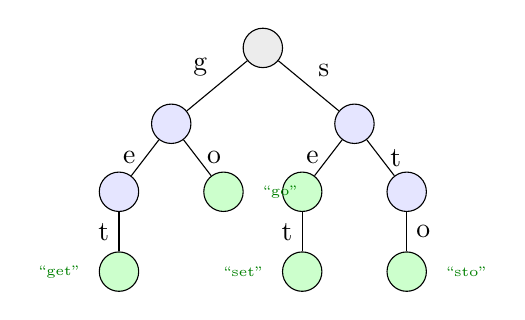
\begin{tikzpicture}[
    >=Stealth,
    tnode/.style={draw, circle, minimum size=0.5cm,
                  font=\tiny\ttfamily, inner sep=1pt},
    every edge/.style={draw, ->, >=Stealth, font=\tiny}
  ]
  \node[tnode, fill=gray!15] (root) {};
  \node[tnode, fill=blue!10, below left=0.6cm and 0.8cm of root] (g) {};
  \node[tnode, fill=blue!10, below right=0.6cm and 0.8cm of root] (s) {};
  \node[tnode, fill=blue!10, below left=0.5cm and 0.3cm of g] (ge) {};
  \node[tnode, fill=green!20, below right=0.5cm and 0.3cm of g] (go) {};
  \node[tnode, fill=green!20, below=0.5cm of ge] (get) {};
  \node[tnode, fill=green!20, below left=0.5cm and 0.3cm of s] (se) {};
  \node[tnode, fill=blue!10, below right=0.5cm and 0.3cm of s] (st) {};
  \node[tnode, fill=green!20, below=0.5cm of se] (set) {};
  \node[tnode, fill=green!20, below=0.5cm of st] (sto) {};

  \draw (root) -- node[above left] {g} (g);
  \draw (root) -- node[above right] {s} (s);
  \draw (g) -- node[left] {e} (ge);
  \draw (g) -- node[right] {o} (go);
  \draw (ge) -- node[left] {t} (get);
  \draw (s) -- node[left] {e} (se);
  \draw (s) -- node[right] {t} (st);
  \draw (se) -- node[left] {t} (set);
  \draw (st) -- node[right] {o} (sto);

  \node[font=\tiny, right=0.1cm of go, text=green!50!black] {``go''};
  \node[font=\tiny, left=0.1cm of get, text=green!50!black] {``get''};
  \node[font=\tiny, left=0.1cm of set, text=green!50!black] {``set''};
  \node[font=\tiny, right=0.1cm of sto, text=green!50!black] {``sto''};
\end{tikzpicture}
\end{center}

\vspace{0.3em}
\begin{alertblock}{Design Goal}
Provide a nibble-based trie with a \textbf{static node pool},
$O(2L)$ insert/search (where $L$ = key length in bytes),
\textbf{zero heap usage}, and prefix-aware lookup.
\end{alertblock}
\end{column}
\end{columns}
\end{frame}

% ===========================================================================
\section{Data Structure}
% ===========================================================================

\begin{frame}[fragile]{The Nibble Trie: 4-Bit Branching}
\begin{columns}[T]
\begin{column}{0.48\textwidth}
\begin{lstlisting}[style=cstyle,
  title={ds/trie/tiku\_kits\_ds\_trie.h}]
#ifndef TIKU_KITS_DS_TRIE_MAX_NODES
#define TIKU_KITS_DS_TRIE_MAX_NODES 64
#endif

#define TIKU_KITS_DS_TRIE_CHILDREN 16
#define TIKU_KITS_DS_TRIE_INVALID  0xFFFF

struct tiku_kits_ds_trie_node {
    uint16_t children[
        TIKU_KITS_DS_TRIE_CHILDREN];
    tiku_kits_ds_elem_t value;
    uint8_t has_value;  /* end-of-key */
};

struct tiku_kits_ds_trie {
    struct tiku_kits_ds_trie_node
        pool[TIKU_KITS_DS_TRIE_MAX_NODES];
    uint16_t pool_next;  /* free index  */
    uint16_t count;      /* stored keys */
};
\end{lstlisting}
\end{column}

\begin{column}{0.48\textwidth}
\textbf{Nibble decomposition:}\\
Each byte of the key is split into two 4-bit nibbles.
Each nibble selects one of 16 children.

\vspace{0.5em}
\begin{center}
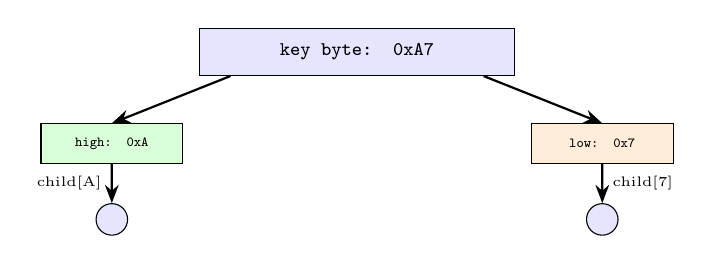
\begin{tikzpicture}[>=Stealth, scale=0.8]
  % Byte box
  \node[draw, minimum width=4cm, minimum height=0.6cm,
        fill=blue!10, font=\scriptsize\ttfamily] (byte) {key byte: 0xA7};

  % Split into nibbles
  \node[draw, minimum width=1.8cm, minimum height=0.5cm,
        fill=green!15, font=\tiny\ttfamily, below left=0.6cm and 0.2cm of byte] (hi)
    {high: 0xA};
  \node[draw, minimum width=1.8cm, minimum height=0.5cm,
        fill=orange!15, font=\tiny\ttfamily, below right=0.6cm and 0.2cm of byte] (lo)
    {low: 0x7};

  \draw[->, thick] (byte.south west) ++(0.5, 0) -- (hi.north);
  \draw[->, thick] (byte.south east) ++(-0.5, 0) -- (lo.north);

  % Nodes
  \node[draw, circle, minimum size=0.4cm, fill=blue!10,
        font=\tiny, below=0.5cm of hi] (n1) {};
  \node[draw, circle, minimum size=0.4cm, fill=blue!10,
        font=\tiny, below=0.5cm of lo] (n2) {};

  \draw[->, thick] (hi) -- node[left, font=\tiny] {child[A]} (n1);
  \draw[->, thick] (lo) -- node[right, font=\tiny] {child[7]} (n2);
\end{tikzpicture}
\end{center}

\vspace{0.3em}
\begin{block}{Why Nibbles (4-bit)?}
\begin{itemize}
  \item 16 children per node (not 256)
  \item Each byte = 2 lookups (depth doubles)
  \item 75\% less memory per node vs.\ byte trie
  \item Good balance of depth vs.\ fan-out
\end{itemize}
\end{block}
\end{column}
\end{columns}
\end{frame}

% ===========================================================================
\section{Return Codes}
% ===========================================================================

\begin{frame}[fragile]{Shared Return Codes}
\begin{columns}[T]
\begin{column}{0.48\textwidth}
\begin{lstlisting}[style=cstyle,
  title={ds/tiku\_kits\_ds.h (shared)}]
typedef int32_t tiku_kits_ds_elem_t;

#define TIKU_KITS_DS_OK          0
#define TIKU_KITS_DS_ERR_NULL   -1
#define TIKU_KITS_DS_ERR_FULL   -2
#define TIKU_KITS_DS_ERR_EMPTY  -3
#define TIKU_KITS_DS_ERR_PARAM  -4
#define TIKU_KITS_DS_ERR_NOTFOUND -5
#define TIKU_KITS_DS_ERR_BOUNDS -6
\end{lstlisting}
\end{column}

\begin{column}{0.48\textwidth}
\begin{block}{Used by the Trie Module}
\begin{itemize}
  \item \texttt{ERR\_NULL} --- NULL pointer or key argument
  \item \texttt{ERR\_FULL} --- node pool exhausted during insert
  \item \texttt{ERR\_PARAM} --- zero-length key
  \item \texttt{ERR\_NOTFOUND} --- key not present in trie
\end{itemize}
\end{block}

\vspace{0.3em}
\begin{alertblock}{Pool Exhaustion}
Unlike arrays or queues, the trie can run out of nodes
mid-insert. \texttt{ERR\_FULL} signals that
\texttt{TIKU\_KITS\_DS\_TRIE\_MAX\_NODES} is too small for
the workload. Increase at compile time.
\end{alertblock}
\end{column}
\end{columns}
\end{frame}

% ===========================================================================
\section{API Reference}
% ===========================================================================

\begin{frame}[fragile]{Complete API}
\begin{table}
\centering
\small
\begin{tabular}{@{}lp{8cm}@{}}
\toprule
\textbf{Function} & \textbf{Description} \\
\midrule
\texttt{\_trie\_init(t)}
  & Initialize node pool; root = node 0, pool\_next = 1 \\
\texttt{\_trie\_insert(t, key, len, val)}
  & Insert key (byte array of \texttt{len}) with associated value;
    allocates nodes from pool as needed \\
\texttt{\_trie\_search(t, key, len, \&val)}
  & Look up key; returns value via pointer or \texttt{ERR\_NOTFOUND} \\
\texttt{\_trie\_contains(t, key, len)}
  & Returns 1 if key exists with a value, 0 otherwise \\
\texttt{\_trie\_remove(t, key, len)}
  & Mark key's terminal node as having no value;
    does not reclaim nodes \\
\midrule
\texttt{\_trie\_count(t)}
  & Return number of stored key-value pairs \\
\texttt{\_trie\_clear(t)}
  & Re-initialize entire pool; reset pool\_next and count \\
\bottomrule
\end{tabular}
\end{table}

\vspace{0.3em}
{\scriptsize All functions are prefixed with \texttt{tiku\_kits\_ds}.
Every function validates pointer arguments and returns \texttt{ERR\_NULL} on failure.}

\begin{alertblock}{Lazy Deletion}
\texttt{remove()} clears the \texttt{has\_value} flag but does not free nodes.
Nodes are only reclaimed by \texttt{clear()}, which resets the entire trie.
This avoids complex tree compaction on resource-constrained MCUs.
\end{alertblock}
\end{frame}

% ===========================================================================
\section{Code Examples}
% ===========================================================================

\begin{frame}[fragile]{Example 1: Command Table Lookup}
\begin{lstlisting}[style=cstyle,
  title={Map CLI command strings to handler IDs}]
#include "tikukits/ds/trie/tiku_kits_ds_trie.h"

#define CMD_GET   1
#define CMD_SET   2
#define CMD_RESET 3
#define CMD_STATUS 4

static struct tiku_kits_ds_trie cmd_trie;

void cmd_table_init(void) {
    tiku_kits_ds_trie_init(&cmd_trie);

    tiku_kits_ds_trie_insert(&cmd_trie, (const uint8_t *)"get",    3, CMD_GET);
    tiku_kits_ds_trie_insert(&cmd_trie, (const uint8_t *)"set",    3, CMD_SET);
    tiku_kits_ds_trie_insert(&cmd_trie, (const uint8_t *)"reset",  5, CMD_RESET);
    tiku_kits_ds_trie_insert(&cmd_trie, (const uint8_t *)"status", 6, CMD_STATUS);
}

int cmd_dispatch(const char *input, uint16_t len) {
    tiku_kits_ds_elem_t handler_id;
    if (tiku_kits_ds_trie_search(&cmd_trie, (const uint8_t *)input, len,
                                  &handler_id) == TIKU_KITS_DS_OK) {
        return (int)handler_id;  /* dispatch to handler */
    }
    return -1;  /* unknown command */
}
\end{lstlisting}
\end{frame}

% ---------------------------------------------------------------------------
\begin{frame}[fragile]{Example 2: Sensor ID to Channel Mapping}
\begin{columns}[T]
\begin{column}{0.48\textwidth}
\begin{lstlisting}[style=cstyle,
  title={Map sensor string IDs to ADC channels}]
#include "tiku_kits_ds_trie.h"

static struct tiku_kits_ds_trie
    sensor_map;

void sensor_map_init(void) {
    tiku_kits_ds_trie_init(&sensor_map);

    /* Register sensors */
    tiku_kits_ds_trie_insert(
        &sensor_map,
        (const uint8_t *)"temp", 4, 0);
    tiku_kits_ds_trie_insert(
        &sensor_map,
        (const uint8_t *)"humi", 4, 1);
    tiku_kits_ds_trie_insert(
        &sensor_map,
        (const uint8_t *)"pres", 4, 2);
    tiku_kits_ds_trie_insert(
        &sensor_map,
        (const uint8_t *)"light", 5, 3);
}

int sensor_get_channel(
    const char *id, uint16_t len)
{
    tiku_kits_ds_elem_t ch;
    if (tiku_kits_ds_trie_search(
            &sensor_map,
            (const uint8_t *)id, len,
            &ch) == TIKU_KITS_DS_OK)
        return (int)ch;
    return -1;
}
\end{lstlisting}
\end{column}

\begin{column}{0.48\textwidth}
\begin{center}
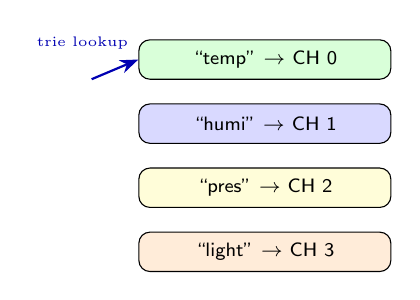
\begin{tikzpicture}[
    >=Stealth,
    entry/.style={draw, rounded corners, minimum width=3.2cm,
                  minimum height=0.5cm, font=\scriptsize\sffamily}
  ]
  \node[entry, fill=green!15] (e1) {``temp'' $\rightarrow$ CH 0};
  \node[entry, fill=blue!15, below=0.3cm of e1] (e2) {``humi'' $\rightarrow$ CH 1};
  \node[entry, fill=yellow!15, below=0.3cm of e2] (e3) {``pres'' $\rightarrow$ CH 2};
  \node[entry, fill=orange!15, below=0.3cm of e3] (e4) {``light'' $\rightarrow$ CH 3};

  \draw[->, thick, blue!70!black] (-2.2, -0.25) -- (e1.west)
    node[above left, font=\tiny] {trie lookup};
\end{tikzpicture}
\end{center}

\vspace{0.5em}
\begin{block}{Advantage over Hash Table}
\begin{itemize}
  \item Prefix queries: find all sensors starting with ``te''
  \item No hash collisions --- worst case is still $O(2L)$
  \item Ordered iteration possible
  \item Shared prefixes save memory
\end{itemize}
\end{block}

\begin{alertblock}{String Keys}
The trie treats keys as raw byte arrays.
String keys work naturally --- no hashing
step, no collision resolution.
\end{alertblock}
\end{column}
\end{columns}
\end{frame}

% ===========================================================================
\section{Embedded Use Cases}
% ===========================================================================

\begin{frame}[fragile]{Use Case: CLI Command Parser with Trie-Based Dispatch}
\begin{columns}[T]
\begin{column}{0.52\textwidth}
\begin{lstlisting}[style=cstyle,
  title={UART CLI with trie-based command dispatch}]
#include "tiku_kits_ds_trie.h"

#define CMD_HELP    10
#define CMD_READ    20
#define CMD_WRITE   30
#define CMD_REBOOT  40
#define CMD_READ_ALL 50

static struct tiku_kits_ds_trie cli;

void cli_init(void) {
    tiku_kits_ds_trie_init(&cli);
    tiku_kits_ds_trie_insert(&cli,
        (const uint8_t *)"help", 4,
        CMD_HELP);
    tiku_kits_ds_trie_insert(&cli,
        (const uint8_t *)"read", 4,
        CMD_READ);
    tiku_kits_ds_trie_insert(&cli,
        (const uint8_t *)"readall", 7,
        CMD_READ_ALL);
    tiku_kits_ds_trie_insert(&cli,
        (const uint8_t *)"write", 5,
        CMD_WRITE);
    tiku_kits_ds_trie_insert(&cli,
        (const uint8_t *)"reboot", 6,
        CMD_REBOOT);
}

void cli_process(const char *line,
                 uint16_t len)
{
    tiku_kits_ds_elem_t cmd;
    if (tiku_kits_ds_trie_search(&cli,
            (const uint8_t *)line, len,
            &cmd) == TIKU_KITS_DS_OK) {
        execute_command((int)cmd);
    } else {
        uart_print("Unknown command\r\n");
    }
}
\end{lstlisting}
\end{column}

\begin{column}{0.44\textwidth}
\begin{center}
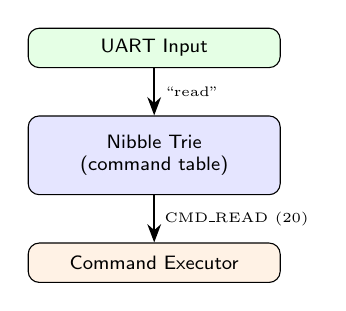
\begin{tikzpicture}[>=Stealth, node distance=0.4cm]
  \node[draw, rounded corners, fill=green!10,
        minimum width=3.2cm, minimum height=0.5cm,
        font=\scriptsize\sffamily] (uart) {UART Input};
  \node[draw, rounded corners, fill=blue!10,
        minimum width=3.2cm, minimum height=1.0cm,
        font=\scriptsize\sffamily, below=0.6cm of uart,
        align=center] (trie)
    {Nibble Trie\\(command table)};
  \node[draw, rounded corners, fill=orange!10,
        minimum width=3.2cm, minimum height=0.5cm,
        font=\scriptsize\sffamily, below=0.6cm of trie] (exec)
    {Command Executor};

  \draw[->, thick] (uart) -- node[right, font=\tiny] {``read''} (trie);
  \draw[->, thick] (trie) -- node[right, font=\tiny] {CMD\_READ (20)} (exec);
\end{tikzpicture}
\end{center}

\vspace{0.5em}
\begin{block}{Why Trie for CLI?}
\begin{itemize}
  \item ``read'' and ``readall'' share prefix nodes
  \item Lookup time depends on command length, not table size
  \item Adding new commands does not affect existing lookup speed
  \item No rehashing when table grows
\end{itemize}
\end{block}

\begin{alertblock}{Prefix Sharing}
Keys ``read'' and ``readall'' share 8 nibble
nodes. A hash table would store them independently.
\end{alertblock}
\end{column}
\end{columns}
\end{frame}

% ===========================================================================
\section{Memory Layout}
% ===========================================================================

\begin{frame}{Memory Layout and Sizing}
\begin{columns}[T]
\begin{column}{0.48\textwidth}
\begin{center}
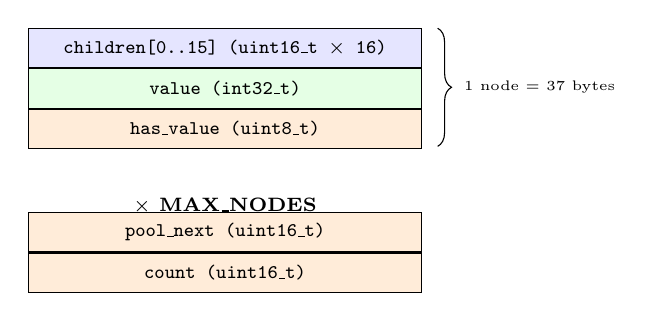
\begin{tikzpicture}[>=Stealth, node distance=0.0cm]
  \node[draw, minimum width=5cm, minimum height=0.5cm,
        fill=blue!10, font=\scriptsize\ttfamily] (c0) {children[0..15] (uint16\_t $\times$ 16)};
  \node[draw, minimum width=5cm, minimum height=0.5cm,
        fill=green!10, font=\scriptsize\ttfamily, below=0cm of c0] (val) {value (int32\_t)};
  \node[draw, minimum width=5cm, minimum height=0.5cm,
        fill=orange!15, font=\scriptsize\ttfamily, below=0cm of val] (hv) {has\_value (uint8\_t)};

  \draw[decorate, decoration={brace, amplitude=5pt}]
    (2.7, 0.25) -- (2.7, -1.25)
    node[midway, right=6pt, font=\tiny] {1 node = 37 bytes};

  \node[font=\scriptsize\bfseries, below=0.5cm of hv] (pool) {$\times$ MAX\_NODES};

  \node[draw, minimum width=5cm, minimum height=0.5cm,
        fill=orange!15, font=\scriptsize\ttfamily, below=0.8cm of hv] (pn)
    {pool\_next (uint16\_t)};
  \node[draw, minimum width=5cm, minimum height=0.5cm,
        fill=orange!15, font=\scriptsize\ttfamily, below=0cm of pn] (cnt) {count (uint16\_t)};
\end{tikzpicture}
\end{center}
\end{column}

\begin{column}{0.48\textwidth}
\begin{block}{Size Formula}
\[
  \text{Per node} = 16 \times 2 + 4 + 1 = 37 \text{ bytes}
\]
\[
  \text{Total} = N \times 37 + 4 \text{ bytes}
\]
\end{block}

\begin{table}
\centering
\scriptsize
\begin{tabular}{@{}rrr@{}}
\toprule
\textbf{MAX\_NODES} & \textbf{Total (bytes)} & \textbf{Approx.\ Keys} \\
\midrule
16  & 596    & 3--5 short keys \\
32  & 1{,}188  & 6--10 short keys \\
64  & 2{,}372  & 12--20 short keys \\
128 & 4{,}740  & 25--40 short keys \\
\bottomrule
\end{tabular}
\end{table}

\vspace{0.3em}
\begin{alertblock}{Memory vs.\ Alphabet Tradeoff}
Nibble trie (16 children) uses 37 bytes/node vs.\
a byte trie (256 children) at 517 bytes/node.
The cost is 2$\times$ depth. For embedded systems,
this tradeoff strongly favors nibbles.
\end{alertblock}
\end{column}
\end{columns}
\end{frame}

% ===========================================================================
\section{Complexity}
% ===========================================================================

\begin{frame}{Time and Space Complexity}
\begin{columns}[T]
\begin{column}{0.48\textwidth}
\begin{table}
\centering
\begin{tabular}{@{}lcc@{}}
\toprule
\textbf{Operation} & \textbf{Best} & \textbf{Worst} \\
\midrule
\texttt{init}     & $O(N)$ & $O(N)$ \\
\texttt{insert}   & $O(2L)$ & $O(2L)$ \\
\texttt{search}   & $O(2L)$ & $O(2L)$ \\
\texttt{contains} & $O(2L)$ & $O(2L)$ \\
\texttt{remove}   & $O(2L)$ & $O(2L)$ \\
\texttt{count}    & $O(1)$ & $O(1)$ \\
\texttt{clear}    & $O(N)$ & $O(N)$ \\
\bottomrule
\end{tabular}
\end{table}

\vspace{0.3em}
{\scriptsize $L$ = key length in bytes, $N$ = \texttt{MAX\_NODES}.\\
$2L$ because each byte produces 2 nibble lookups.}
\end{column}

\begin{column}{0.48\textwidth}
\begin{block}{Space Complexity}
\[
  O(N \times 16) \text{ memory for } N \text{ nodes}
\]
\begin{itemize}
  \item Worst case: each key consumes $2L$ new nodes
  \item Best case: keys share prefix nodes
  \item Shared prefixes significantly reduce node usage
\end{itemize}
\end{block}

\vspace{0.3em}
\begin{block}{Key Property}
\begin{itemize}
  \item Lookup time depends \textbf{only} on key length
  \item Independent of number of stored keys
  \item No degradation as table fills up
  \item Compare: hash table degrades at high load
\end{itemize}
\end{block}
\end{column}
\end{columns}

\vspace{0.5em}
\begin{alertblock}{Deterministic Timing}
Every insert/search/remove takes exactly $2L$ node traversals.
No collisions, no probing, no rebalancing --- ideal for
real-time embedded applications.
\end{alertblock}
\end{frame}

% ===========================================================================
\section{Test Suite}
% ===========================================================================

\begin{frame}{Test Cases Overview}
\begin{table}
\centering
\small
\begin{tabular}{@{}clp{7cm}@{}}
\toprule
\textbf{\#} & \textbf{Test Function} & \textbf{What It Verifies} \\
\midrule
1 & \texttt{test\_kits\_ds\_trie\_init}
  & Initialization, pool reset, count is zero \\
2 & \texttt{test\_kits\_ds\_trie\_insert\_search}
  & Insert 3 keys, search returns correct values \\
3 & \texttt{test\_kits\_ds\_trie\_contains}
  & Contains returns 1 for present keys, 0 for absent \\
4 & \texttt{test\_kits\_ds\_trie\_remove}
  & Remove clears value, search returns NOTFOUND, count decrements \\
5 & \texttt{test\_kits\_ds\_trie\_prefix\_sharing}
  & Keys with shared prefix reuse nodes, pool usage is efficient \\
6 & \texttt{test\_kits\_ds\_trie\_overwrite}
  & Re-insert same key updates value, count unchanged \\
7 & \texttt{test\_kits\_ds\_trie\_pool\_exhaustion}
  & Insert until pool full, returns ERR\_FULL \\
8 & \texttt{test\_kits\_ds\_trie\_clear\_reset}
  & Clear resets pool, trie is reusable \\
9 & \texttt{test\_kits\_ds\_trie\_null\_inputs}
  & All functions reject NULL with ERR\_NULL \\
\bottomrule
\end{tabular}
\end{table}
\end{frame}

% ===========================================================================
\section{Summary}
% ===========================================================================

\begin{frame}{Summary}
\begin{columns}[T]
\begin{column}{0.48\textwidth}
\begin{block}{What We Built}
\begin{itemize}
  \item Nibble-based trie (4-bit branching)
  \item 7 API functions: init, insert, search, contains, remove, count, clear
  \item $O(2L)$ insert/search/remove
  \item Static node pool --- zero heap usage
  \item Lazy deletion (clear-flag, no compaction)
\end{itemize}
\end{block}

\begin{block}{Key Design Choices}
\begin{itemize}
  \item 4-bit nibbles: 16 children per node
  \item Static pool of pre-allocated nodes
  \item Keys are raw byte arrays (string-friendly)
  \item Shared prefixes reduce memory usage
  \item Pool size tunable at compile time
\end{itemize}
\end{block}
\end{column}

\begin{column}{0.48\textwidth}
\begin{block}{Use Cases}
\begin{itemize}
  \item CLI command parsing and dispatch
  \item Sensor ID to channel mapping
  \item AT command lookup tables
  \item Register mnemonic resolution
  \item Any prefix-aware string lookup
\end{itemize}
\end{block}

\begin{block}{Files}
\scriptsize
\begin{tabular}{@{}lp{4.5cm}@{}}
Common: & \texttt{ds/tiku\_kits\_ds.h} \\
Header: & \texttt{ds/trie/tiku\_kits\_ds\_trie.h} \\
Source: & \texttt{ds/trie/tiku\_kits\_ds\_trie.c} \\
Tests:  & \texttt{tests/ds/test\_kits\_ds\_trie.c} \\
\end{tabular}
\end{block}
\end{column}
\end{columns}
\end{frame}

% ---------------------------------------------------------------------------
\begin{frame}{Thank You}
\begin{center}
\Large\textbf{TikuKits DS: Trie}\\[0.5em]
\normalsize Nibble Trie for Prefix-Aware Lookup on Embedded Systems\\[1.5em]

\begin{tabular}{rl}
  Repository: & \url{https://github.com/tikuos/tikuOS} \\
  License:    & Apache 2.0 \\
  Common:     & \texttt{tikukits/ds/tiku\_kits\_ds.h} \\
  Header:     & \texttt{tikukits/ds/trie/tiku\_kits\_ds\_trie.h} \\
  Source:     & \texttt{tikukits/ds/trie/tiku\_kits\_ds\_trie.c} \\
  Tests:      & \texttt{tikukits/tests/ds/test\_kits\_ds\_trie.c} \\
\end{tabular}
\end{center}
\end{frame}

\end{document}
